\section{Local response to a larger budget}\label{sec:localredistribution}
\paragraph{Question and definition.} Reducing an aggregate position error need not improve every feature. For a fixed feature $i$ at the same time $t$, let $e_{i,t}(\varepsilon)=|x_{i,t}(\varepsilon)-q_{i,t}|/L$ and $\Delta e_{i,t}=e_{i,t}(\varepsilon_b)-e_{i,t}(\varepsilon_a)$, where $\varepsilon_a<\varepsilon_b$. Positive changes mean worsening. These compare budgets, not motion between time steps. Define $R_h=\#\{(i,t):\Delta e_{i,t}>h\}/N$. For the same feature--frame population,
\[
 E_{\mathrm{pool}}(\varepsilon_b)-E_{\mathrm{pool}}(\varepsilon_a)=N^{-1}\sum_{i,t}\Delta e_{i,t}.
\]
Positive and negative local changes can therefore coexist while their mean decreases.

\begin{figure}[ht]
\centering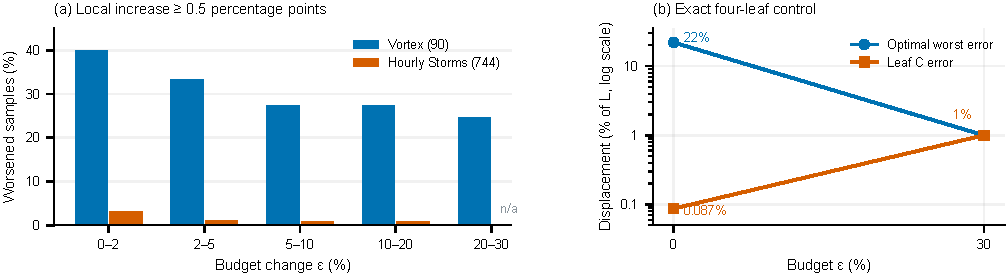
\includegraphics[width=\linewidth]{figures/fig_local_redistribution.pdf}
\caption{Local response to larger merge budgets. (a) Percentage of fixed feature--frame observations whose position error increases by at least 0.5 percentage points of the canvas. Vortex has 90 frames; the separate hourly Storms diagnostic has 744. Hourly Storms has no 30\% result (n/a). These cohorts do not replace the seven-sequence benchmark and do not isolate dimensionality. (b) An exhaustive four-leaf control: the optimal maximum displacement falls from 22\% to 1\%, while leaf C's error rises from 0.087\% to 1\%. The vertical scale is logarithmic.}\label{fig:localresponse}
\end{figure}

\paragraph{Nested feasibility and pointwise error.} With input, reference, interval geometry and any externally imposed position cap fixed, increasing the merge budget enlarges the feasible set. The globally minimal worst displacement cannot increase, but may plateau. This is a statement about an optimal value, not a componentwise inequality between the errors of two selected layouts. The implemented order search is also heuristic and its secondary objective balances geometry and temporal behavior. The following control separates the pointwise issue from both heuristic search and temporal history.

\paragraph{Exhaustive control.} Use a static four-leaf join tree: leaf values zero, sibling pairs $\{A,B\}$ and $\{C,D\}$ merging at 0.4, root at 1. Set $L=\Delta_F=1$, references $q=(0.20,0.80,0.18,0.60)$, widths $W_i=0.06$, gap $g=0.01$, anchor slack $\rho=0.5$ and $\beta=0$. Source centres are $(q_i,y_i)$ with $y=(0.144,0.156,0.146,0.052)$. Enumerate all 24 orders and independently solve the minimax placement LP for each, using the canvas, interval, separation and anchor-slack constraints. Among minimax-optimal orders, minimize the same fixed convex secondary objective with reference, geometry and eccentricity weights 4, 1 and 0.1, and no temporal term. A $10^{-9}L$ allowance is used only for numerical cap feasibility; independent LP first-order oracles certify convex QP gaps below $10^{-8}$.

At $\varepsilon=0$, eight exact orders are eligible. The unique minimax-optimal order is $C,D,A,B$ with $\tau^*=0.22$. The reference-hull/width bound is $(0.60-0.20+0.04)/2=0.22$. At $\varepsilon=0.30$, all 24 orders are eligible. The unique minimax-optimal order is $C,A,D,B$ with $\tau^*=0.01$. The references of C and A are separated by 0.02, but their anchors require separation $(1-\rho)W+g=0.04$, certifying the lower bound $(0.04-0.02)/2=0.01$. Feasible placements attain both bounds. Original and relaxed barriers are $(0.4,1,0.4)$ and $(0.7,0.7,0.7)$; all six labelled pairwise merge errors are remeasured. C's selected errors are 0.000868919 and 0.010000001, i.e., 0.087\% and 1\% of $L$. Thus strict improvement of the exact global minimax value need not improve every point. This constructed counterexample establishes lack of guarantee, not prevalence.

\paragraph{Additional diagnostic cohorts.} Vortex uses 90 original $128^3$ normalized scalar fields, 111--156 retained extrema per frame and 12,446 feature--frame observations. Its supplied scalar range is $[-1,1]$; the join convention uses $-f/2$. A fixed 2\% persistence simplification precedes layout and differs from the budget. References are fixed X voxel coordinates on $L=127$. The hourly Storms diagnostic uses 744 hourly ERA5 anomaly fields for December 1999 on the retained $49\times49$ analysis grid, with 1--12 retained minima per frame (3,502 observations). The anomaly subtracts a centred 192-hour per-location background; spatial processing and reference are unchanged. This differs from the main paper's 118 half-day Storms sequence. These separately prepared cohorts are not added to the 917-frame cross-method population. Physical feature identity beyond the saved computational matching is not assumed.

Both use the frozen certified order/optimal-barrier/capped-QP construction, fixed widths, gaps, references and feature sets, with $B_t=\tau_t+\beta$. Vortex budgets are $\{0,0.02,0.05,0.10,0.20,0.30\}$; hourly Storms uses $\{0,0.02,0.05,0.10,0.20\}$. Comparisons pair the same feature at the same time, never by proximity after layout. The additional 30\% Vortex run covers all 90 frames from the initial frame, preserving temporal history, and passed independent source-tree, interval, cap, profile and sampled-LP checks. This audit remeasures saved continuous anchors; no layout or solver weight was tuned for its results.

\paragraph{Reporting thresholds.} Changes beyond $10^{-6}L$ are classified as positive or negative; the rest are unchanged. Increases of at least 0.005 and 0.01 of $L$ (0.5 and 1 percentage points) are also reported. These are numerical reporting thresholds, not calibrated perceptual limits. Counts are descriptive: repeated features and times are not treated as independent trials, and no inferential confidence intervals are claimed. Table~\ref{tab:localresponse} reports all adjacent budget changes.

\begin{table}[ht]\centering\small
\caption{Fixed-population budget comparisons. $N$ is feature--frame observations per transition. ``Worse'' uses $\Delta e>10^{-6}$; pp means absolute percentage points of $L$.}\label{tab:localresponse}
\begin{tabular}{llrrrr}\toprule
Cohort & $\varepsilon_a\to\varepsilon_b$ & $N$ & Worse (\%) & $\ge0.5$ pp (\%) & $\ge1$ pp (\%)\\\midrule
\csname @@input\endcsname tables/tab_local_response.tex
\bottomrule\end{tabular}\end{table}

At 20\% to 30\% on Vortex, pooled error falls from 8.794\% to 4.273\%, and the sequence maximum from 30.769\% to 28.741\%, but 3,847 of 12,446 observations worsen (30.91\%); 3,077 worsen by at least 0.5 percentage points (24.72\%). Restricting to the 88 frames whose mean and maximum both strictly decrease leaves 12,141 observations, of which 3,778 worsen (31.12\%). The effect is therefore not explained solely by frames whose overall position error worsens. Local increases also occur with an unchanged order at that time (13 observations in this transition); different temporal histories can affect a fixed-order QP, so this is not a causal decomposition of order and temporal effects.

\begin{figure}[ht]
\centering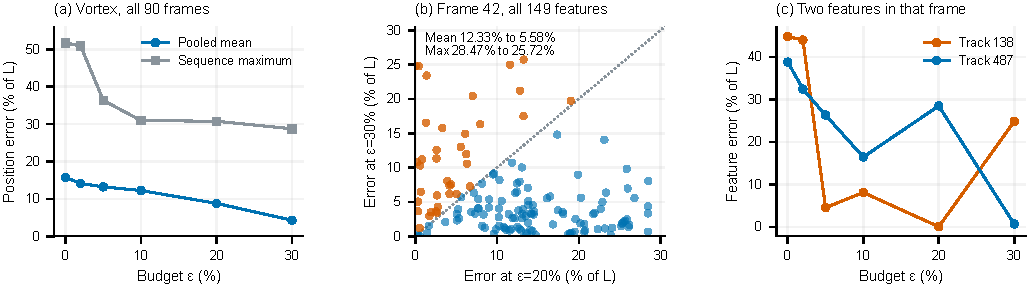
\includegraphics[width=\linewidth]{figures/fig_local_redistribution_detail.pdf}
\caption{Vortex response to changing budget. (a) Pooled and maximum errors over all 90 frames. (b) All 149 features at frame 42, comparing 20\% and 30\%. Orange indicates an increase of at least 0.5 percentage points; points above the diagonal worsen. Both frame mean and maximum decrease. (c) Two features from that frame: track 138 worsens and track 487 improves from 20\% to 30\%. The frame is selected by the largest local increase among frames whose mean and maximum both decrease; it illustrates an extreme, not typical behavior.}\label{fig:localdetail}
\end{figure}

\paragraph{Illustrative case and interpretation.} At frame 42 (zero-based), track 138's error grows from 0.031\% to 24.800\% of $L$ from 20\% to 30\%, although the frame mean falls from 12.332\% to 5.579\% and the maximum from 28.467\% to 25.719\%. The case-selection rule is explicit in Fig.~\ref{fig:localdetail}; full-population counts, not this extreme, support prevalence statements. An analyst choosing a budget for a feature of interest should inspect its signed local response alongside aggregate displacement and hierarchy-error disclosure. This diagnostic changes no certified constraint and claims no pointwise improvement guarantee.

\paragraph{Precision example retained from the main text.} The data resolution should match field precision. On Cylinder, whose saddles are nearly degenerate, $\nu^*$ is 12.24\% when only exactly equal levels are merged and 6.15\% at $\varepsilon_0=10^{-6}$; part of this hierarchy lies below data precision. This precision control differs from increasing the analyst budget with a fixed feature population.

\paragraph{Reproduction.} Run \nolinkurl{code/experiments/local_redistribution/run.py}, then \texttt{control.py} and \texttt{plot.py} in that directory. Bound compressed inputs, SHA256 manifests, all 76,238 pointwise transition records, summaries and the 24-order control are in \nolinkurl{code/results/local_redistribution20261030/}. Inputs contain continuous anchors, references, stable track IDs and orders; this audit needs no external volume archive and does not rerun the original volume extraction.
